\documentclass[12pt,letterpaper,titlepage]{article}

\usepackage{fontspec}
\defaultfontfeatures{Mapping=tex-text}
\usepackage{xunicode}
\usepackage{xltxtra}
\usepackage{amsmath}
\usepackage{pdfpages}
\usepackage{amsfonts}
\usepackage{amssymb}
\setcounter{secnumdepth}{0}
\usepackage{nameref}
\usepackage{enumitem}
\usepackage{environ}

\setmainfont{Times New Roman}
\showboxdepth=\maxdimen
\showboxbreadth=\maxdimen


\usepackage{paracol}
\usepackage{wrapfig}
\globalcounter{table}
\globalcounter{figure}
\usepackage{graphicx}
\usepackage[left=1in,right=1in,top=1in,bottom=1in]{geometry}
\graphicspath{{img/}}

\author{Jacob Abel}
\title{	Homework 3
	\\\large ECE2004 CRN:12898
}

\setlength{\parskip}{0.5em}

\begin{document}
\maketitle
\begin{raggedright}

\paragraph{Question 1: }

Solve for the voltages at node A and node B.

\begin{center}
\includegraphics[width=.75\textwidth, height=\textheight, keepaspectratio=true]{hw3q1}
\end{center}

\begin{align*}
    \frac{A-10V}{1k\Omega} + \frac{A-B}{2k\Omega} + \frac{A}{0.5k\Omega} =& 0
\\  \frac{B-A}{2k\Omega} + \frac{B}{4k\Omega} - 1mA =& 0
\\  7A - B =& 20V
\\  3B - 2A =& 4V
\\  7A - 20V =& B
\\  A =& \frac{64}{19}V\approx 3.37V
\\  B =& \frac{68}{19}V\approx 3.58V
\end{align*}

\clearpage

\paragraph{Question 2: }

Solve for $i$.

\begin{center}
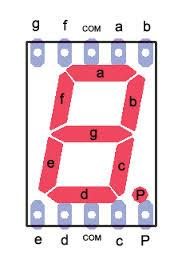
\includegraphics[width=.75\textwidth, height=\textheight, keepaspectratio=true]{hw3q2}
\end{center}

\begin{align*}
    \frac{10V-B}{100\Omega} + \frac{10V-A}{10\Omega} - i =& 0
\\  \frac{A-10V}{10\Omega} + \frac{A}{20\Omega} + \frac{A-B}{30\Omega}=& 0
\\  \frac{B-10V}{100\Omega} + \frac{B-A}{30\Omega} + 0.02A =& 0
\\  \frac{B + 10A}{100\Omega} =& 1.1A - i
\\  11A - 2B =& 60V
\\  13B - 4A =& 30V
\\  \frac{11}{2}A - 30V =& B
\\  \frac{56}{9}V =& A
\\  \frac{38}{9}V =& B
\\  \frac{299}{450}A =& 1.1A - i
\\  i =& \frac{98}{255}A \approx 0.435A 
\end{align*}

\clearpage

\paragraph{Question 3: }

Solve for $i_x$. (Hint: Super nodes may contain more than two nodes.)

\begin{center}
\includegraphics[width=\textwidth, height=\textheight, keepaspectratio=true]{hw3q3}
\end{center}

\begin{align*}
    v_1 + 5V=& v_2
\\  v_1 + 20V=& v_3
\\  \frac{v_1 - 10V}{4\Omega} + \frac{v_1}{8\Omega} + i_x + \frac{v_3-10V}{4\Omega}=& 0
\\  i_x=& -\frac{5v_1}{8\Omega}
\\  \frac{v_1+5V}{16\Omega} + \frac{5v_1}{8\Omega} =& 0
\\  \frac{5V + 11v_1}{16\Omega} =& 0
\\  v_1 =& \frac{-5}{11}V
\\  i_x=& -\frac{5\frac{-5}{11}V}{8\Omega}
\\  i_x=& \frac{25}{88}A \approx 0.284A
\end{align*}

\clearpage

\paragraph{Question 4: }

\begin{center}
\includegraphics[width=0.9\textwidth, height=\textheight, keepaspectratio=true]{hw3q4}
\end{center}

\begin{enumerate}[label=\Alph*)]
\item Use Mesh Current Analysis to solve for $I_1$ and $I_2$.

\begin{align*}
    1\Omega(I_1) + 8\Omega(I_1-I_2) + 10V - 10V =& 0
\\  8\Omega(I_2-I_1) + 9\Omega(I_2) - 5V + 10V =& 0
\\  I_1(9\Omega)-8\Omega(I_2) =& 0
\\  I_2(17\Omega) - 8\Omega(I_1) + 5V =& 0
\\  I_1 =& \frac{8}{9}I_2
\\  \frac{89\Omega}{9}I_2 + 5V =& 0
\\  I_2 =& -\frac{45}{89}A \approx -0.506A
\\  I_1 =& -\frac{40}{89}A \approx -0.449A
\end{align*}

\item What is the value of the current through the $8\Omega$ resistor, $i_x$, and in what direction is it flowing?
\begin{align*}
    i_x + I_2 - I_1 =& 0
\\  i_x =& I_1 - I_2
\\  i_x =& -\frac{40}{89}A +\frac{45}{89}A
\\  i_x =& \frac{5}{89}A \approx 0.056A
\end{align*}

$i_x$ is flowing towards ground (aka in the same direction as the arrow on the diagram for $i_x$ is pointing.)

\end{enumerate}

\end{raggedright}
\end{document}
